% Results on the official FD001 test set (issue #7). Every number comes from
% results/metrics/fd001_test.json and fd001_test_capped125.json; figures are
% written by notebooks/phase1/04_ml_results.ipynb.

\section{Results}
\label{sec:results}

All results are on the official FD001 test set: 100 engines, each scored once at
its last recorded cycle against the uncapped true RUL, unless stated otherwise.
The cross-validated configurations behind them are in
Table~\ref{tab:model_selection}.

\begin{table}[!t]
\centering
\caption{Official FD001 test results (100 engines, last cycle, uncapped RUL).
Stage columns give the RMSE on the 33 late, 34 mid and 33 early engines. Lower
is better; bold marks the best of the six models in each column.}
\label{tab:test_results}
\setlength{\tabcolsep}{4pt}
\begin{tabular}{lrrrrrr}
\hline
Model & RMSE & MAE & NASA & Late & Mid & Early \\
\hline
\multicolumn{7}{l}{\emph{Engineered features (Phase~1 method)}} \\
Random Forest & 27.55 & \textbf{17.67} & 145{,}410 & 7.52 & \textbf{25.76} & 39.49 \\
XGBoost       & 30.50 & 19.82 & 61{,}202  & \textbf{5.62} & 29.62 & 43.39 \\
Elastic Net   & 28.39 & 23.57 & 7{,}777   & 24.78 & 32.60 & \textbf{27.09} \\
\hline
\multicolumn{7}{l}{\emph{Raw inputs (comparison)}} \\
Random Forest & \textbf{26.15} & 19.22 & 8{,}414 & 13.50 & 27.94 & 32.95 \\
XGBoost       & 26.84 & 19.19 & 7{,}002 & 14.32 & 28.50 & 33.77 \\
Elastic Net   & 31.08 & 25.80 & \textbf{6{,}903} & 29.71 & 32.08 & 31.38 \\
\hline
\end{tabular}
\end{table}

\subsection{Overall Test Error}
Table~\ref{tab:test_results} lists the six models. With the engineered features,
the Phase~1 method, Random Forest reaches an RMSE of 27.55 cycles and an MAE of
17.67 cycles, the lowest MAE of all six models. No model is best on every
metric: Random Forest on raw inputs has the lowest RMSE (26.15), and the raw
Elastic Net the lowest NASA score. The engineered features lower RMSE only for
the Elastic Net (31.08 to 28.39) and raise it for both tree models, by 1.4
cycles for Random Forest and 3.7 for XGBoost. All six RMSEs lie within five
cycles of each other on a single set of 100 engines without confidence
intervals, so we do not read them as a ranking. Test RMSE
(26--31) is well below CV RMSE (36--42) because cross-validation scores every
training cycle, including RUL values far above the test range
(Section~\ref{sec:methodology}).

\subsection{Error by Degradation Stage}
The overall numbers hide two opposite effects (Table~\ref{tab:test_results},
Fig.~\ref{fig:stage_rmse}). Near failure, on the 33 engines with $y\le 50$, the
engineered features roughly halve the tree models' error: Random Forest falls
from 13.50 to 7.52 and XGBoost from 14.32 to 5.62. This is the stage in which
maintenance is scheduled, and where the rolling means and slopes track the
accelerating degradation described in Section~\ref{sec:dataset_eda}. On the 33
engines with $y>100$, the engineered tree models are worse than their raw
counterparts (Random Forest 39.49 against 32.95, XGBoost 43.39 against 33.77).
The Elastic Net shows the reverse pattern: its late-stage RMSE of 24.78 is the
worst of the engineered models, because a linear function cannot follow the
sharp fall of RUL at the end of life, but it is the most accurate early.

\begin{figure}[!t]
\centering
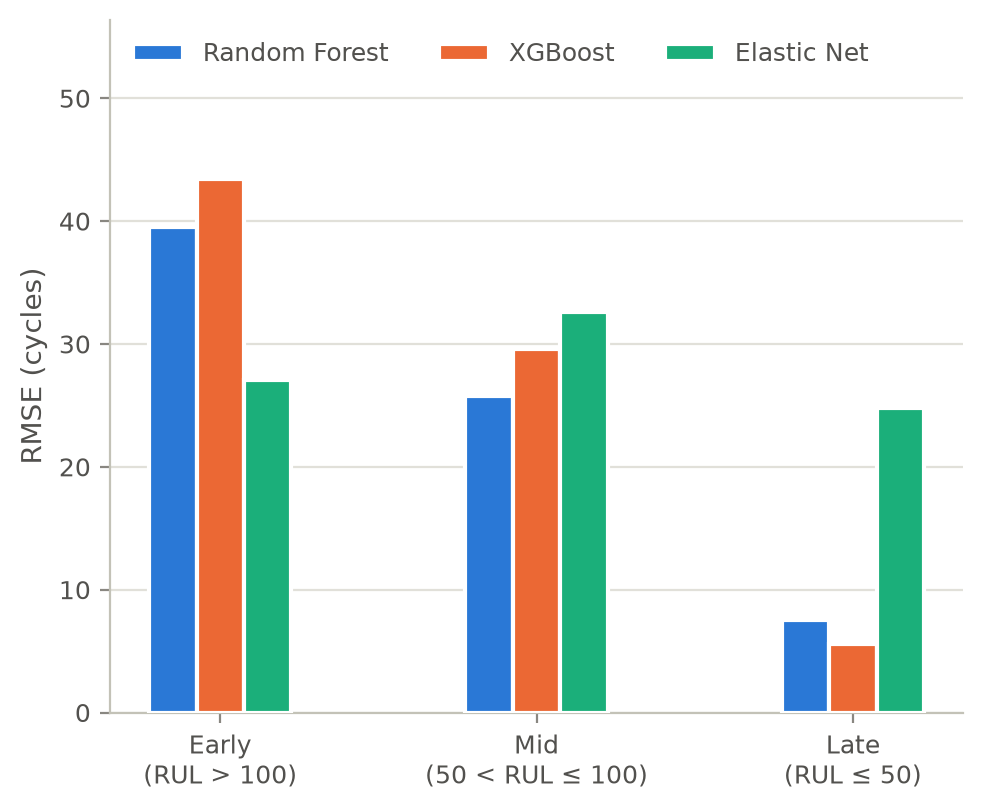
\includegraphics[width=0.92\columnwidth]{../../results/figures/fd001_test_stage_rmse.png}
\caption{Test RMSE by degradation stage of the true RUL for the engineered
models.}
\label{fig:stage_rmse}
\end{figure}

The early-stage errors are mostly overestimates. An engine whose sensors still
look healthy receives a long predicted life, typical of training engines that
lived 128 to 362 cycles, yet no test engine had more than 145 cycles left at its
last observed cycle. The engineered Random Forest overestimates 9 engines by more
than 50 cycles. Tree SHAP attributes far more of each engineered prediction to
\texttt{cycle} than to any sensor feature (Section~\ref{sec:models}), so for
young engines the models fall back on an age-based estimate and overestimate
their remaining life. Capping the training target roughly halves this error: the
engineered Random Forest's early-stage RMSE falls from 39.49 to 20.05 cycles,
still scored against the uncapped test RUL (Section~\ref{sec:capped}).

\begin{figure*}[!t]
\centering
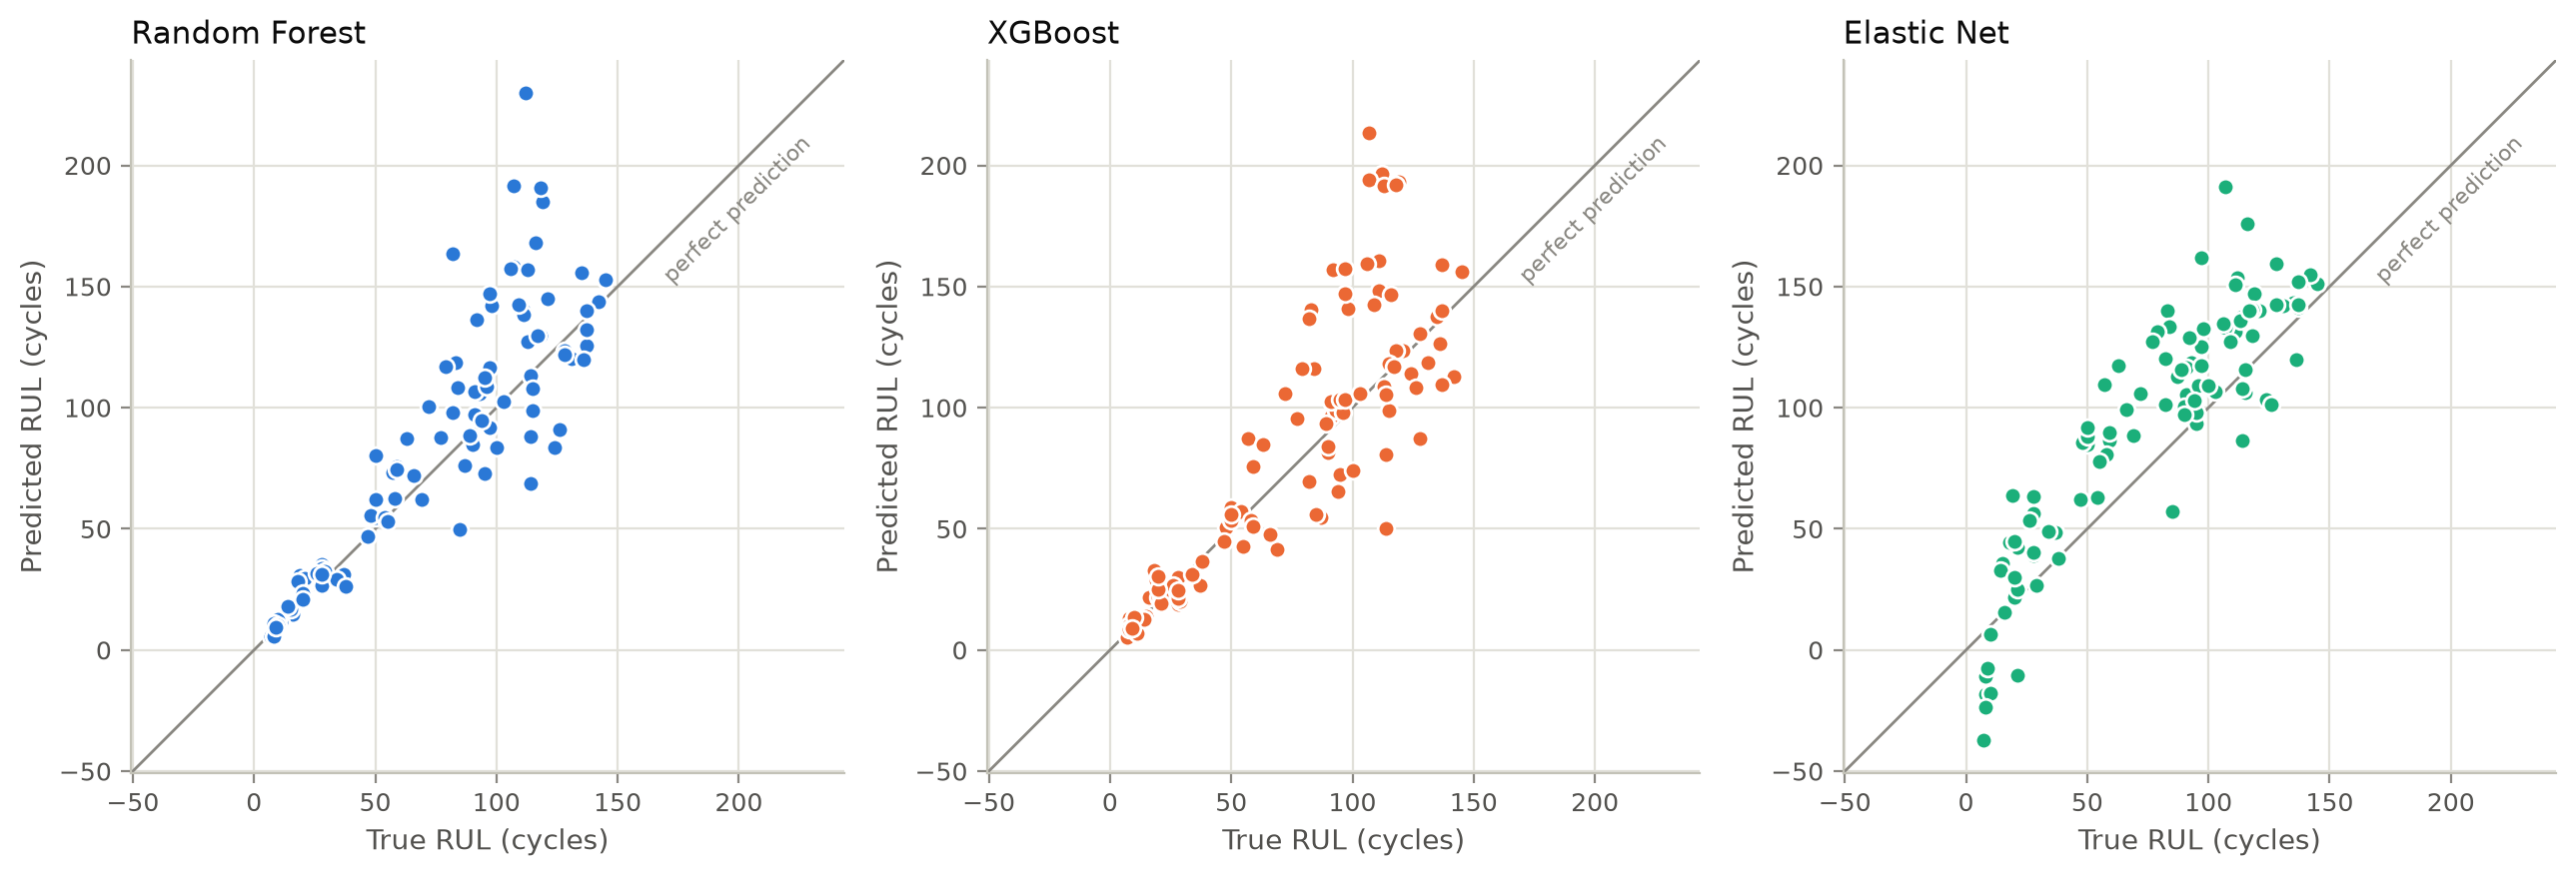
\includegraphics[width=\textwidth]{../../results/figures/fd001_test_pred_vs_true.png}
\caption{Predicted against true RUL at the last cycle of each test engine for the
engineered models. Points above the diagonal predict more life than the engine
had. The panels share one scale so that the Elastic Net's negative predictions
remain visible.}
\label{fig:pred_vs_true}
\end{figure*}

\subsection{Per-Engine Predictions}
Fig.~\ref{fig:pred_vs_true} shows the same pattern engine by engine: the
predictions are tight below about 50 cycles of true RUL and spread widely above
about 80. The Elastic Net predicts negative RUL for 7 test engines, since its
output is not bounded; the predictions are reported without clipping.
Fig.~\ref{fig:trajectories} follows the engineered Random Forest over the whole
recorded history of the four test engines observed longest, chosen by history
length rather than by error. These engines started with 270 to 330 cycles of
life, more than most training engines had, and early in each record the
prediction stays far below the true RUL. The gap narrows as degradation becomes
visible: at the last cycle, engines 49 and 62 are predicted within one cycle,
while engines 91 and 93 remain underestimated by 12 and 35 cycles, an early and
therefore safe error.

\begin{figure*}[!t]
\centering
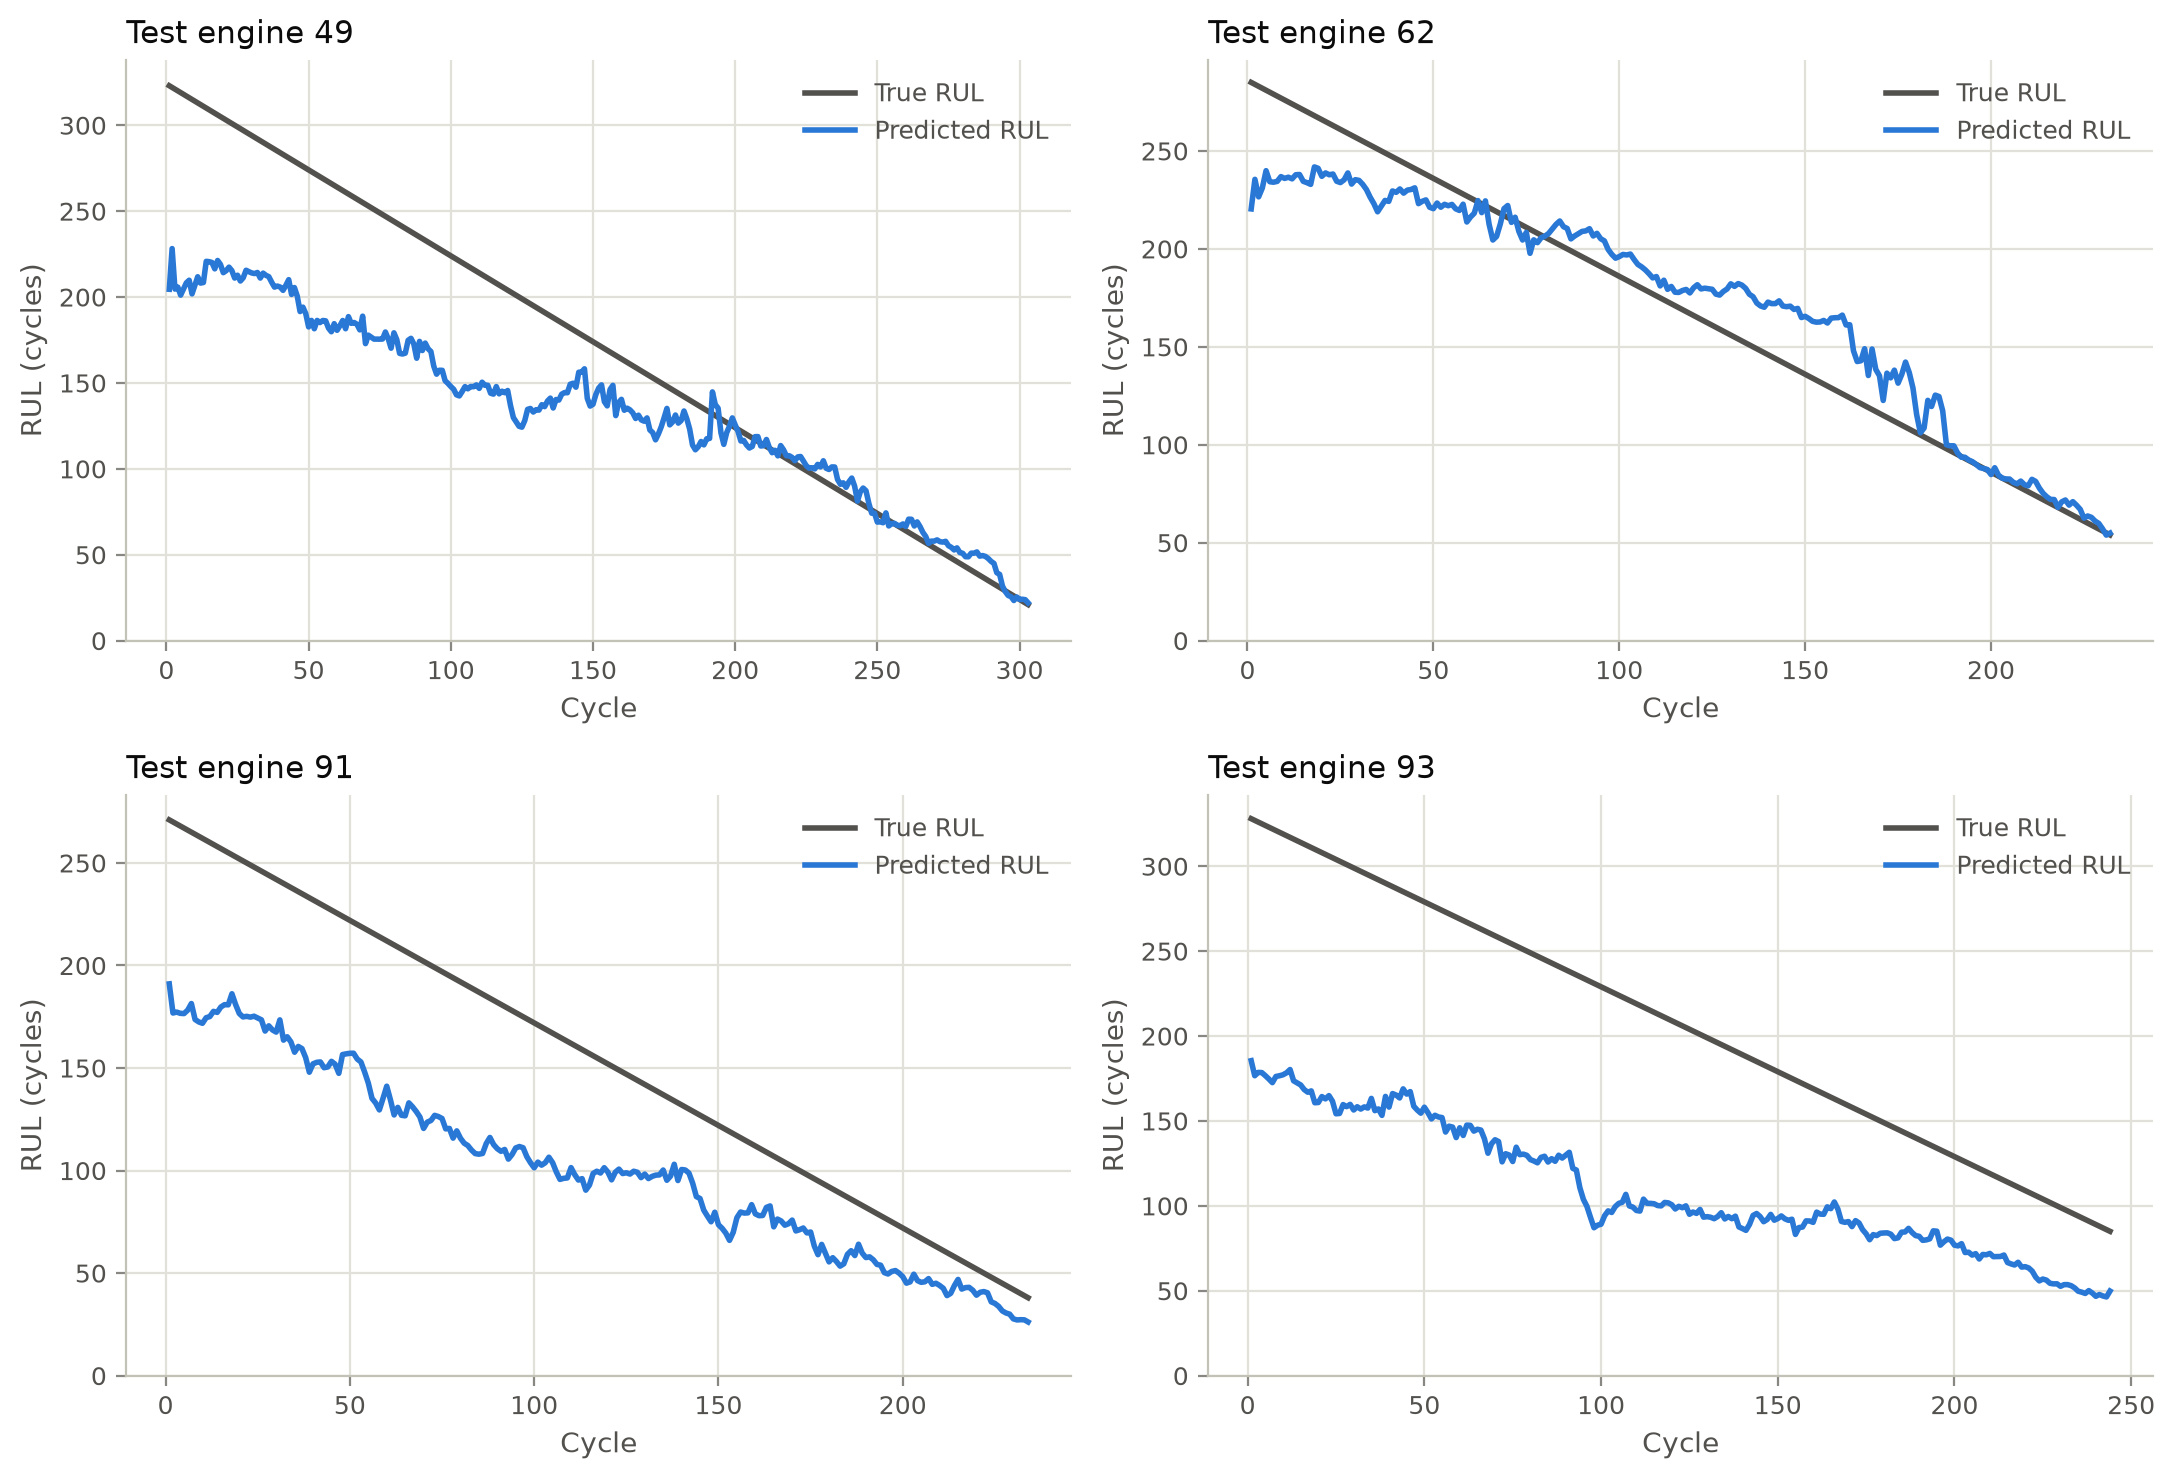
\includegraphics[width=0.78\textwidth]{../../results/figures/fd001_test_trajectories.png}
\caption{Engineered Random Forest predictions over the recorded cycles of the four
test engines with the longest histories (49, 62, 91 and 93), against the true
RUL.}
\label{fig:trajectories}
\end{figure*}

\subsection{Sensitivity of the NASA Score}
Because the NASA score is an exponential sum over engines, single engines
dominate it. Test engine~1 was observed for only 31 cycles and had 112 left; the
engineered Random Forest predicts 230. That one overestimate of 118 cycles
contributes 133{,}652 of the model's 145{,}410, or 92\%, while the other 99
engines add 11{,}758. XGBoost's largest single penalty is 68\% of its score. The
NASA ranking in Table~\ref{tab:test_results} is therefore driven by a handful of
young engines, which is why we read it together with RMSE, MAE and the stage
errors.

\subsection{Capped-Target Check}
\label{sec:capped}
To test whether the uncapped target explains the early-stage errors, Random
Forest was retrained with the training RUL capped at 125 cycles, using the same
grid, folds and seed, and scored against the true, uncapped test RUL
(Table~\ref{tab:capped}). Capping lowers the RMSE of both feature sets and
reverses their order: engineered features now reach 16.21 against 18.66 for raw
inputs, with an early-stage RMSE of 20.05 against 23.12 and a late-stage RMSE of
7.39 against 13.44. The comparison between feature sets therefore depends on how
RUL is defined. This is a single-model check with a cap taken from the
literature, not chosen on the test set; the full ablation over all models, with
the cap justified from training data, belongs to Phase~2.

\begin{table}[!t]
\centering
\caption{Random Forest test RMSE with the uncapped and the capped (125 cycles)
training target, scored against the true, uncapped test RUL.}
\label{tab:capped}
\begin{tabular}{lrr}
\hline
Training target & Engineered & Raw \\
\hline
Uncapped (primary)      & 27.55 & 26.15 \\
Capped at 125 (ablation) & 16.21 & 18.66 \\
\hline
\end{tabular}
\end{table}
